% Système mobile d’imagerie interventionnelle Discovery IGS 730

\section{Présentation du système}
\subsection{Mise en situation}
Développé dans le cadre d’un projet ambitieux associant des industriels (GE Healthcare, BA Systèmes et C\&K), deux laboratoires de recherche (CEA-LIST et IRCCYN) et un centre de recherche
préclinique (laboratoire CR2i INRA AP-HP), le Discovery IGS 730 (figure 1) est le premier système
mobile d’imagerie interventionnelle. Embarquant un ensemble de logiciels de traitement d’images
pour les applications vasculaires, l’oncologie et la cardiologie (figure 2) et permettant un accès complet au patient, il guide les gestes de l’équipe médicale tout au long de l’intervention chirurgicale.

\begin{figure}[!h]
\centering
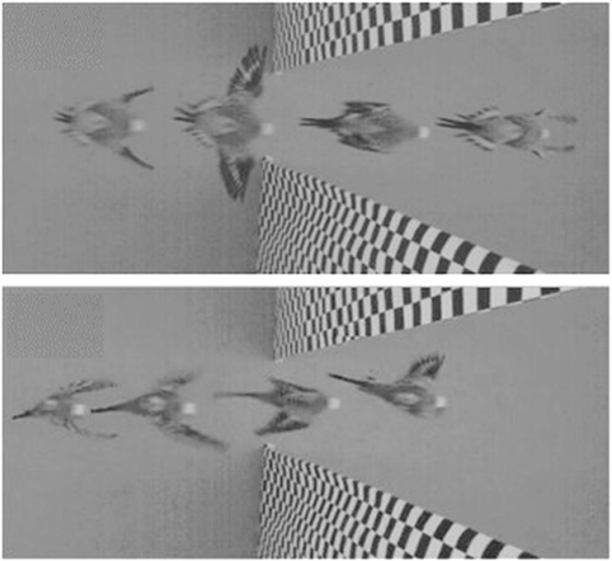
\includegraphics[width=\linewidth]{fig_01}
\caption{\label{fig:01}  Système d’imagerie robotisé Discovery IGS 730 en situation de travail (photo de gauche) et en mode parking (photo de droite).}
\end{figure}


\begin{figure}[!h]
\centering
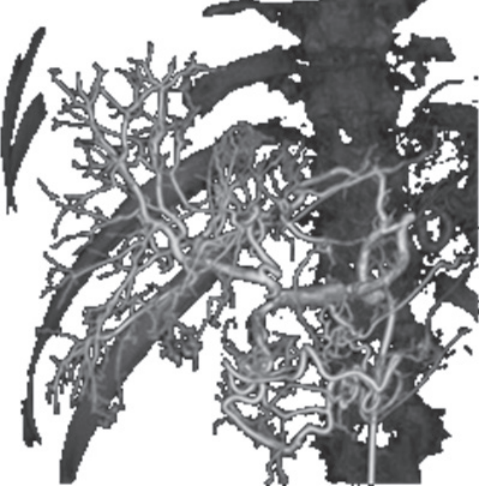
\includegraphics[height=4cm]{fig_02_a}
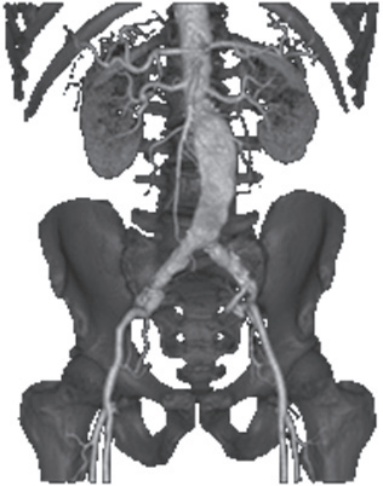
\includegraphics[height=4cm]{fig_02_b}
\caption{\label{fig:02a} Système vasculaire du poumon.}
\caption{\label{fig:02b} Système vasculaire général.}
\caption{\label{fig:02}  Images 3D obtenues avec le système d’imagerie du Discovery IGS 730.}
\end{figure}

Le Discovery IGS 730 révolutionne le domaine de l’imagerie interventionnelle. Contrairement aux
systèmes d’angiographie traditionnels, il n’est ni fixé au sol, ni suspendu au plafond, mais dispose
d’une base motorisée guidée par laser qui transporte l’arceau d’imagerie. Cette innovation technologique offre une mobilité totale au système qui peut, par exemple, rejoindre de manière autonome
une position « parking » prédéfinie afin de laisser tout le champ disponible à l’équipe médicale pour
s’occuper du patient. Ce gain de mobilité permet également une intégration aisée en milieu clinique,
un accès facilité au patient et des possibilités de positionnement illimitées.


\subsection{Analyse système partielle}
La figure 3 présente un extrait du cahier des charges du système d’imagerie dans la phase de vie
d’utilisation. La figure 4 présente son diagramme de définition des blocs.


\begin{figure}[!h]
\centering
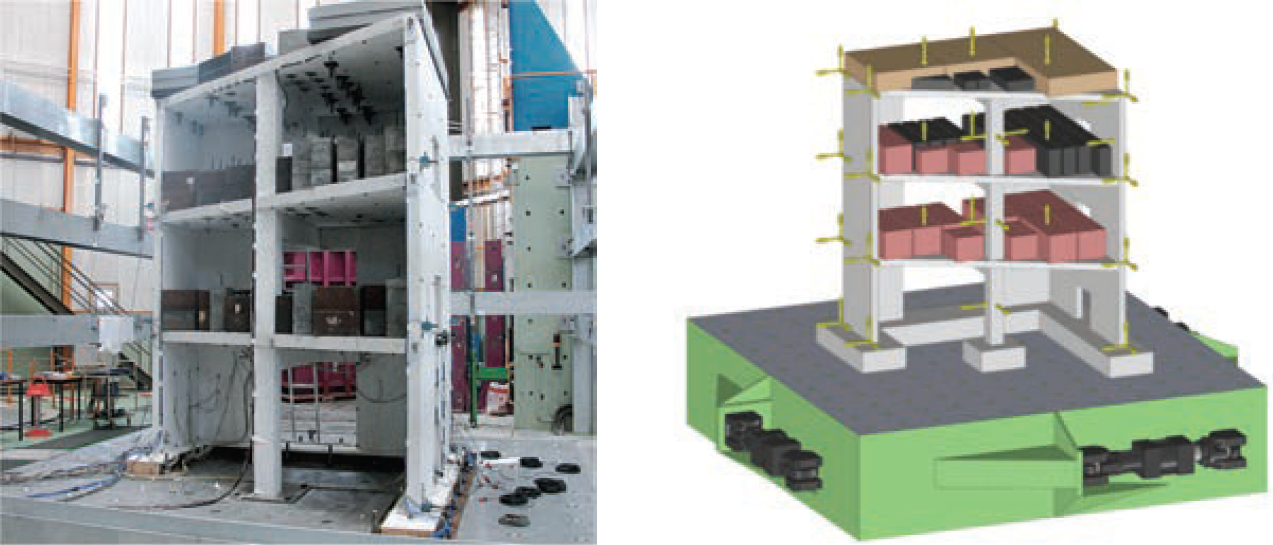
\includegraphics[width=\linewidth]{fig_03}
\caption{\label{fig:03}  Diagramme d’exigences partiel du Discovery IGS 730.}
\end{figure}


\begin{figure}[!h]
\centering
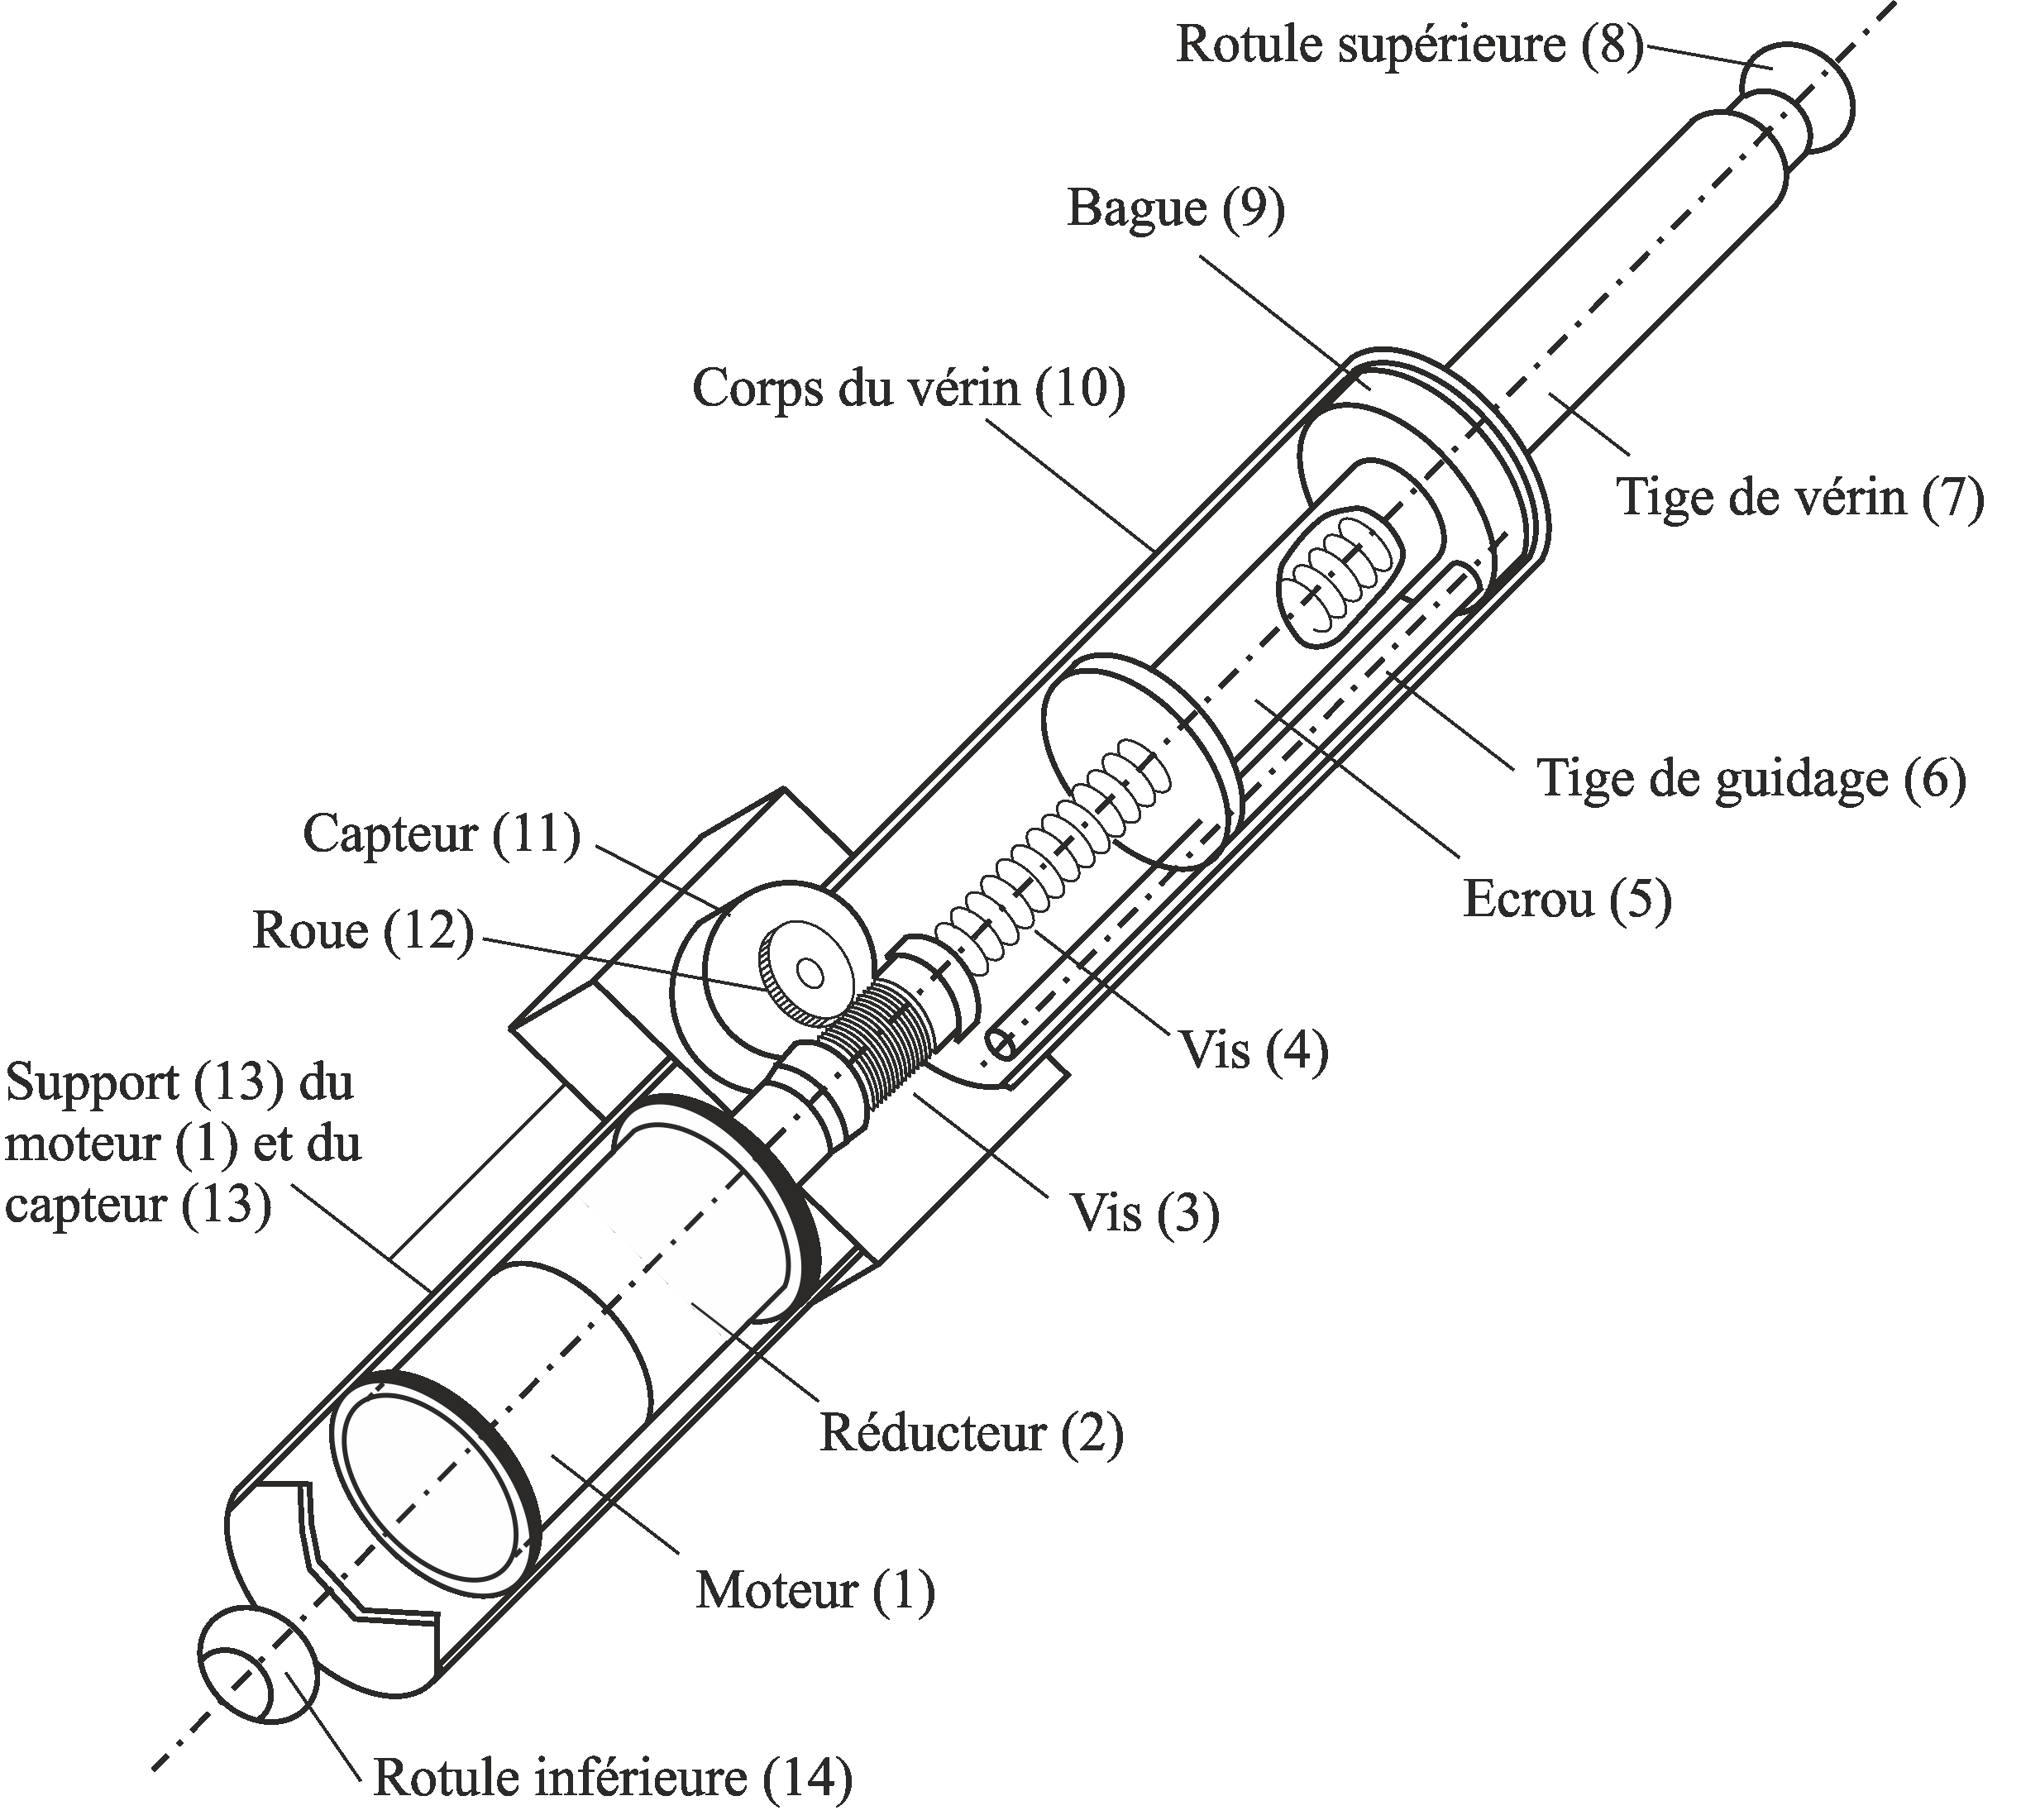
\includegraphics[width=\linewidth]{fig_04}
\caption{\label{fig:04}  Diagramme de définition de blocs du Discovery IGS 730.}
\end{figure}

Le système Discovery IGS 730 est constitué principalement (figure 4, page 3 et figure 5) :
\begin{itemize}
\item d’une base motorisée, aussi appelée AGV (pour Automated Guided Vehicle, soit véhicule à
guidage automatique) ;
\item d’une perche et d’un support de câbles ;
\item du sous-système d’imagerie supporté par un bras en « C » ou arceau. Le système d’imagerie
est lié à la base motorisée par l’intermédiaire de deux liaisons pivot. Un point caractéristique
appelé « isocentre » (point $I_C$) est rattaché au sous-système d’imagerie. Il est défini comme
l’intersection de l’axe optique et de l’axe de la liaison pivot AGV/système pivot.
\end{itemize}

\begin{figure}[!h]
\centering
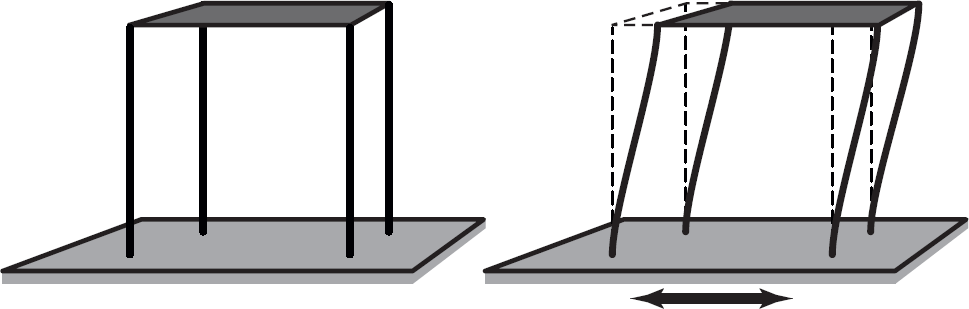
\includegraphics[width=\linewidth]{fig_05}
\caption{\label{fig:05}  Composants du Discovery IGS 730.}
\end{figure}

La base motorisée AGV (figure 6) est constituée :
\begin{itemize}
\item d’une structure support, ou châssis, composée du bras vertical et du cadre Y ;
\item de deux sous-ensembles roue motrice et motorisation associée (un motoréducteur d’orientation et un motoréducteur de propulsion pour chaque roue) ;
\item de deux doubles roues « folles » non motorisées.
\end{itemize}


\begin{figure}[!h]
\centering
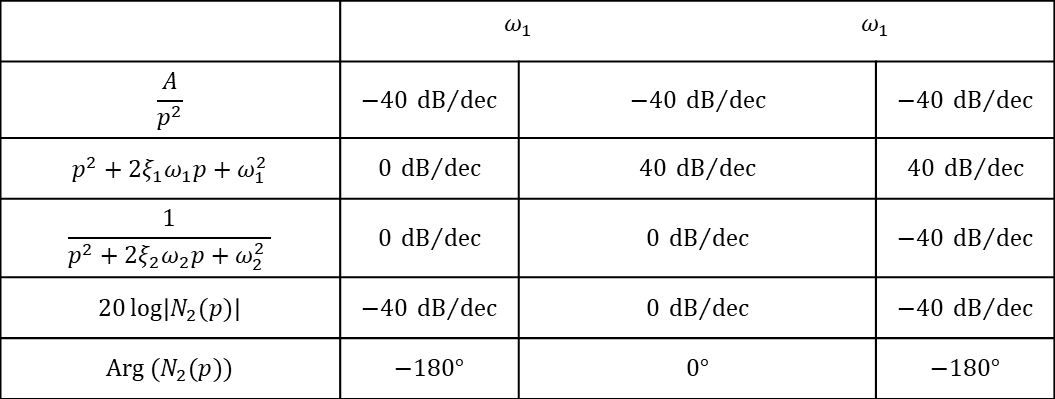
\includegraphics[width=\linewidth]{fig_06}
\caption{\label{fig:06} Éléments du sous-système AGV, carter et sous-système d’imagerie enlevés.}
\end{figure}

\subsection{Problème posé}
La mobilité totale apportée au Discovery IGS 730, véritable innovation technologique dans le domaine de l’imagerie interventionnelle, a conduit les ingénieurs responsables du développement à travailler sur des problématiques spécifiques liées :
\begin{itemize}
\item à la maîtrise du positionnement du sous-système d’imagerie par rapport au patient ;
\item à la sécurité du patient et de l’équipe médicale au cours des déplacements du système dans la
salle d’intervention.
\end{itemize}
\begin{obj}
L’objectif de cette étude est de vérifier certaines performances du système afin de valider partiellement le respect des exigences liées au positionnement de l’AGV et par suite, du sous-système
d’imagerie (Id. 1.1) et à la sécurité des personnes au cours des déplacements (Id. 1.2).
\end{obj}


\subsection{Démarche}

Le respect des exigences relatives au positionnement du sous-système d’imagerie (Id. 1.1), objet de
la partie 2, est abordé à travers les points suivants :
\begin{itemize}
\item étude géométrique et cinématique de l’AGV afin d’estimer la précision requise au niveau de
l’orientation des roues motrices (Id. 1.1.2) ;
\item prévision des performances de la commande associée au mouvement de translation de la base
motorisée (Id. 1.1.3) ;
\item étude de la stratégie de localisation de l’AGV et développement d’algorithmes d’estimation
de sa position (Id. 1.1.1).
\end{itemize}
Le respect des exigences relatives à la sécurité des personnes (Id. 1.2) fait l’objet de la partie 3 consacrée à la prévision du comportement dynamique du système lors d’un freinage d’urgence intervenant
au cours d’une manœuvre de translation (Id. 1.2.1.1).

\section{Validation des exigences relatives au positionnement du sous-système d’imagerie}
\subsection{Modélisation géométrique et cinématique de l’AGV}
\begin{obj}
Vérifier que l’exigence « Précision de positionnement de l’axe de rotation » (Id. 1.1.2.1) peut
être satisfaite.
\end{obj}


Au cours d’une intervention médicale ou de certains examens d’imagerie, l’ensemble du système
est amené à pivoter autour du patient suivant un axe vertical. Afin de ne pas perturber le processus
d’acquisition, la position de l’isocentre $I_C$ par rapport au patient ne doit pas varier durant la manœuvre
(figure 5). Il est donc nécessaire de maîtriser, par le biais de l’orientation des roues motrices, le
positionnement de l’axe de pivotement du système, afin que celui-ci passe par l’isocentre $I_C$.

\subsection*{Paramétrage et hypothèses}

Le modèle géométrique retenu et le paramétrage associé sont donnés sur la figure 7, page 6.

Les repères et angles suivants sont introduits pour l’étude :
\begin{itemize}
\item $\rep{0}$ est un repère attaché à la salle d’intervention. Il a pour origine l’isocentre $I_C$ (supposé fixe
dans la salle) et pour base $\base{x_{0}}{y_{0}}{z_{0}}$ tel que le vecteur $z_{0}$ soit vertical ascendant ;
\item $\rep{C} \repere{I_C}{x_{C}}{y_{C}}{z_{0}}$, repère associé au cadre Y, avec $\psi = \angl{x_{0}}{x_{C}}= \angl{y_{0}}{y_{C}}$ l’angle associé à la
rotation du cadre Y autour de l’axe vertical $\axe{I_C}{z_{0}}$ passant par l’isocentre ;
\item $\rep{P}\repere{A}{x_{P}}{y_{P}}{z_{0}}$ repère associé à la liaison pivot d’axe $\axe{A}{z_{0}}$ de la roue motrice droite avec le
cadre Y, avec $\beta = \angl{x_{C}}{x_{P}}= \angl{y_{C}}{y_{P}}$ l’angle associé à l’orientation de la roue motrice droite
($R_D$) par rapport au cadre Y ;
\item $\rep{R}\repere{A}{x_{R_D}}{y_{P}}{z_{R_D}}$, repère associé à la roue motrice droite ($R_D$), avec $\theta_D = \angl{x_{P}}{x_{R_D}}= \angl{z_{0}}{z_{R_D}}$ 
l’angle associé à la rotation de la roue motrice droite ($R_D$) autour de l’axe $\axe{A}{x_{R_D}}$.
\end{itemize}

L’AGV est animé d’un mouvement de rotation autour de l’axe $\axe{I}{z_0}$; sa géométrie est considérée
comme symétrique par rapport à l’axe $\axe{I}{y_c}$.
Les dimensions utiles ont pour valeurs : $a = \SI{1 440}{mm}$, $e = \SI{800}{mm}$, $r = AI_D = \SI{115}{mm}$.

